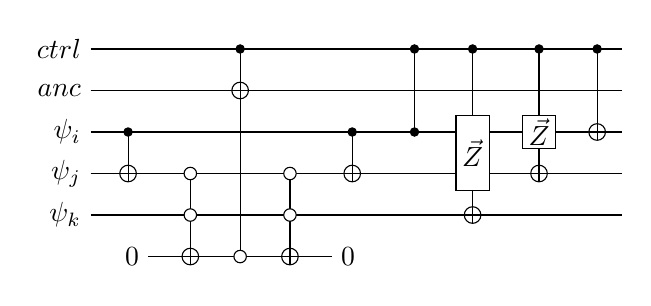
\begin{tikzpicture}[scale=1.000000,x=1pt,y=1pt]
\filldraw[color=white] (0.000000, -7.500000) rectangle (192.000000, 82.500000);
% Drawing wires
% Line 1: ctrl W ctrl
\draw[color=black] (0.000000,75.000000) -- (192.000000,75.000000);
\draw[color=black] (0.000000,75.000000) node[left] {$ctrl$};
% Line 2: anc W anc
\draw[color=black] (0.000000,60.000000) -- (192.000000,60.000000);
\draw[color=black] (0.000000,60.000000) node[left] {$anc$};
% Line 3: i W \psi_i
\draw[color=black] (0.000000,45.000000) -- (192.000000,45.000000);
\draw[color=black] (0.000000,45.000000) node[left] {$\psi_i$};
% Line 4: j W \psi_j
\draw[color=black] (0.000000,30.000000) -- (192.000000,30.000000);
\draw[color=black] (0.000000,30.000000) node[left] {$\psi_j$};
% Line 5: k W \psi_k
\draw[color=black] (0.000000,15.000000) -- (192.000000,15.000000);
\draw[color=black] (0.000000,15.000000) node[left] {$\psi_k$};
% Line 6: c1 W 0 0
\draw[color=black] (13.500000,0.000000) -- (94.500000,0.000000);
% Done with wires; drawing gates
% Line 9: i +j
\draw (13.500000,45.000000) -- (13.500000,30.000000);
\filldraw (13.500000, 45.000000) circle(1.500000pt);
\begin{scope}
\draw[fill=white] (13.500000, 30.000000) circle(3.000000pt);
\clip (13.500000, 30.000000) circle(3.000000pt);
\draw (10.500000, 30.000000) -- (16.500000, 30.000000);
\draw (13.500000, 27.000000) -- (13.500000, 33.000000);
\end{scope}
% Line 10: c1 START
\draw[color=black] (21.000000,0.000000) node[fill=white,left,minimum height=15.000000pt,minimum width=15.000000pt,inner sep=0pt] {\phantom{$0$}};
\draw[color=black] (21.000000,0.000000) node[left] {$0$};
% Line 11: -k -j +c1
\draw (36.000000,30.000000) -- (36.000000,0.000000);
\draw[fill=white] (36.000000, 15.000000) circle(2.250000pt);
\draw[fill=white] (36.000000, 30.000000) circle(2.250000pt);
\begin{scope}
\draw[fill=white] (36.000000, 0.000000) circle(3.000000pt);
\clip (36.000000, 0.000000) circle(3.000000pt);
\draw (33.000000, 0.000000) -- (39.000000, 0.000000);
\draw (36.000000, -3.000000) -- (36.000000, 3.000000);
\end{scope}
% Line 12: ctrl -c1 +anc
\draw (54.000000,75.000000) -- (54.000000,0.000000);
\filldraw (54.000000, 75.000000) circle(1.500000pt);
\draw[fill=white] (54.000000, 0.000000) circle(2.250000pt);
\begin{scope}
\draw[fill=white] (54.000000, 60.000000) circle(3.000000pt);
\clip (54.000000, 60.000000) circle(3.000000pt);
\draw (51.000000, 60.000000) -- (57.000000, 60.000000);
\draw (54.000000, 57.000000) -- (54.000000, 63.000000);
\end{scope}
% Line 13: -k -j +c1
\draw (72.000000,30.000000) -- (72.000000,0.000000);
\draw[fill=white] (72.000000, 15.000000) circle(2.250000pt);
\draw[fill=white] (72.000000, 30.000000) circle(2.250000pt);
\begin{scope}
\draw[fill=white] (72.000000, 0.000000) circle(3.000000pt);
\clip (72.000000, 0.000000) circle(3.000000pt);
\draw (69.000000, 0.000000) -- (75.000000, 0.000000);
\draw (72.000000, -3.000000) -- (72.000000, 3.000000);
\end{scope}
% Line 14: c1 END
\draw[color=black] (87.000000,0.000000) node[fill=white,right,minimum height=15.000000pt,minimum width=15.000000pt,inner sep=0pt] {\phantom{$0$}};
\draw[color=black] (87.000000,0.000000) node[right] {$0$};
% Line 15: i +j
\draw (94.500000,45.000000) -- (94.500000,30.000000);
\filldraw (94.500000, 45.000000) circle(1.500000pt);
\begin{scope}
\draw[fill=white] (94.500000, 30.000000) circle(3.000000pt);
\clip (94.500000, 30.000000) circle(3.000000pt);
\draw (91.500000, 30.000000) -- (97.500000, 30.000000);
\draw (94.500000, 27.000000) -- (94.500000, 33.000000);
\end{scope}
% Line 17: ctrl i
\draw (117.000000,75.000000) -- (117.000000,45.000000);
\filldraw (117.000000, 75.000000) circle(1.500000pt);
\filldraw (117.000000, 45.000000) circle(1.500000pt);
% Line 19: i j G $\vec{Z}$ ctrl +k
\draw (138.000000,75.000000) -- (138.000000,15.000000);
\begin{scope}
\draw[fill=white] (138.000000, 37.500000) +(-45.000000:8.485281pt and 19.091883pt) -- +(45.000000:8.485281pt and 19.091883pt) -- +(135.000000:8.485281pt and 19.091883pt) -- +(225.000000:8.485281pt and 19.091883pt) -- cycle;
\clip (138.000000, 37.500000) +(-45.000000:8.485281pt and 19.091883pt) -- +(45.000000:8.485281pt and 19.091883pt) -- +(135.000000:8.485281pt and 19.091883pt) -- +(225.000000:8.485281pt and 19.091883pt) -- cycle;
\draw (138.000000, 37.500000) node {$\vec{Z}$};
\end{scope}
\filldraw (138.000000, 75.000000) circle(1.500000pt);
\begin{scope}
\draw[fill=white] (138.000000, 15.000000) circle(3.000000pt);
\clip (138.000000, 15.000000) circle(3.000000pt);
\draw (135.000000, 15.000000) -- (141.000000, 15.000000);
\draw (138.000000, 12.000000) -- (138.000000, 18.000000);
\end{scope}
% Line 20: i G $\vec{Z}$ ctrl +j
\draw (162.000000,75.000000) -- (162.000000,30.000000);
\begin{scope}
\draw[fill=white] (162.000000, 45.000000) +(-45.000000:8.485281pt and 8.485281pt) -- +(45.000000:8.485281pt and 8.485281pt) -- +(135.000000:8.485281pt and 8.485281pt) -- +(225.000000:8.485281pt and 8.485281pt) -- cycle;
\clip (162.000000, 45.000000) +(-45.000000:8.485281pt and 8.485281pt) -- +(45.000000:8.485281pt and 8.485281pt) -- +(135.000000:8.485281pt and 8.485281pt) -- +(225.000000:8.485281pt and 8.485281pt) -- cycle;
\draw (162.000000, 45.000000) node {$\vec{Z}$};
\end{scope}
\filldraw (162.000000, 75.000000) circle(1.500000pt);
\begin{scope}
\draw[fill=white] (162.000000, 30.000000) circle(3.000000pt);
\clip (162.000000, 30.000000) circle(3.000000pt);
\draw (159.000000, 30.000000) -- (165.000000, 30.000000);
\draw (162.000000, 27.000000) -- (162.000000, 33.000000);
\end{scope}
% Line 21: ctrl +i
\draw (183.000000,75.000000) -- (183.000000,45.000000);
\filldraw (183.000000, 75.000000) circle(1.500000pt);
\begin{scope}
\draw[fill=white] (183.000000, 45.000000) circle(3.000000pt);
\clip (183.000000, 45.000000) circle(3.000000pt);
\draw (180.000000, 45.000000) -- (186.000000, 45.000000);
\draw (183.000000, 42.000000) -- (183.000000, 48.000000);
\end{scope}
% Done with gates; drawing ending labels
% Done with ending labels; drawing cut lines and comments
% Done with comments
\end{tikzpicture}
